\chapter{System architecture}
\label{ch:architecture}

\lhead{Chapter 7. \emph{System architecture}}

TODO.. introduction


\section{Overview}

Our prototype consists of multiple systems that communicate with each other.
The applications are listed below:

\begin{enumerate}
	\item NIPEN/NIP
	\item Front-end
	\item Heart Rate Application
	\item Weight Application
	\item Weight Polling Service
\end{enumerate}

NIPEN or NIP is our server application that consists of an API and a database.
This application is capable of receiving weight and heart rate data and store them in a database.
It is also able to retrieve data from the database and then send it to our front-end, which then visualizes the information sent.
The next three applications are able to send information to NIP.
For instance the heart rate application is capable of measuring a heart rate and then send it to the integration platform.
The two weight applications are able to fetch weight data from HealthVault and send it to NIP.
The main difference between them is that the \textit{Weigh Application} runs on an Android device, while the \textit{Weight Polling Service} runs on a server or a computer.
In figure \ref{figure:abstract-architecture} an abstract architecture is given of how our applications communicate with each other.

\begin{figure}[h]
\centering
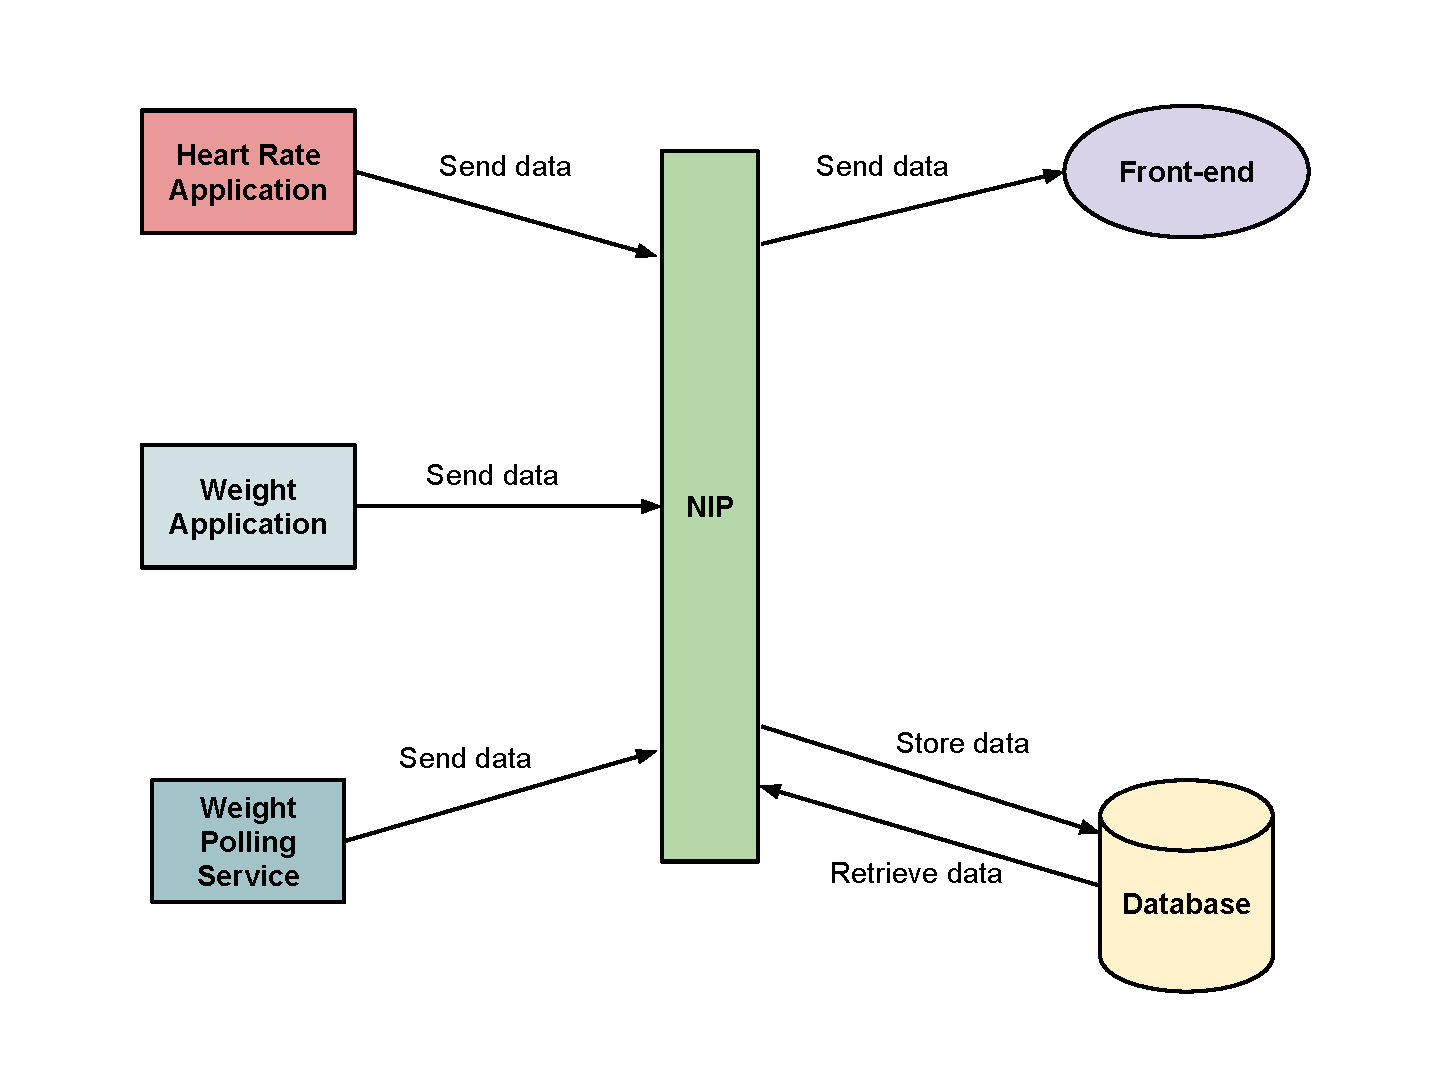
\includegraphics[scale=0.5]{../Figures/abstract-architecture.pdf}
\caption{Abstract architecture}
\label{figure:abstract-architecture}
\end{figure}

\section{NIPEN}

NIPEN is an integration platform for two data types, namely heart rate and weight.
By using the HTTP methods GET and POST it is possible to retrieve and store data into NIP, respectively.
This data needs to be stored in a... 

TODO

\textbf{System architecture}

\begin{figure}[h]
\centering
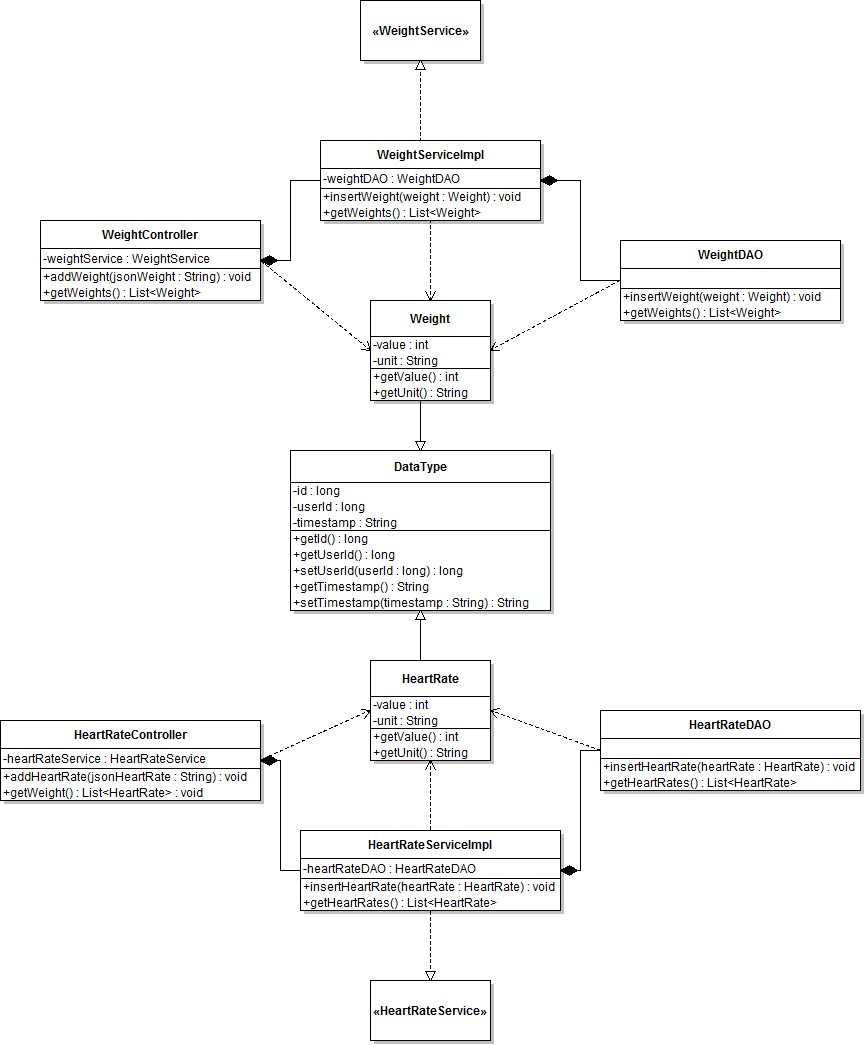
\includegraphics[scale=0.5]{../Figures/NIPEN-class-diagram.png}
\caption{NIPEN class diagram}
\label{figure:nipen-class-diagram}
\end{figure}

TODO

\textbf{Data format}

We are using JSON strings when transmitting data to and from the server.
The representation of the data is inspired from the Human API.
Both heart rate and weight data is represented with the same attributes.
They contain an ID, user ID, time stamp, value and a unit.
The ID is not needed, when the JSON string is sent, because it is created on the server side.
Below is a representation of a heart rate JSON string that can be used to store heart rate data on the server:

\begin{verbatim}
{
    "userId":1,
    "timestamp":"2013-10-27 14:57:39.0",
    "value":65,
    "unit":"bpm"
}
\end{verbatim}

A weight measurement can be sent in the same format but should be sent with another unit.
The ID of the data is shown when receiving the data from the server:

\begin{verbatim}
{
    "id":39,
    "userId":1,
    "timestamp":"2013-10-27 14:57:39.0",
    "value":65,
    "unit":"bpm"
}
\end{verbatim} 

\textbf{API calls}

It supports HTTP GET request to the following addresses:

%\begin{enumerate}
	%\item <server address>/nipen/api/human/heart_rates
	%\item <server address>/nipen/api/human/weights
%\end{enumerate}

By performing one of the HTTP GET request, mentioned above, it is possible to receive the data for the specified data type.

TODO

\textbf{Database}

We are using a MySQL database for data storage.
It consists of two tables for each data type, one for heart rate and one for weight.
The heart rate table is shown in figure \ref{figure:heart-rate-database-diagram} and the weight table in figure \ref{figure:weight-database-diagram}. 
As we can see the tables are identical the only difference is the name.
The reason we didn't merge this tables is to separate the data, and it is also more efficient.
It would require more resources to separate the data if they all were in one table.

\begin{figure}[h]
\centering
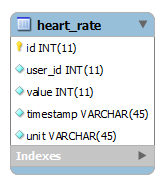
\includegraphics[scale=1.0]{../Figures/heart-rate-database-diagram.png}
\caption{Heart rate database diagram}
\label{figure:heart-rate-database-diagram}
\end{figure}

\begin{figure}[h]
\centering
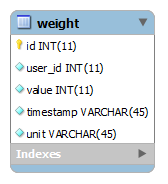
\includegraphics[scale=1.0]{../Figures/weight-database-diagram.png}
\caption{Weight database diagram}
\label{figure:weight-database-diagram}
\end{figure}

We have created separate classes for accessing the database through our server application.
One for heart rate (HeartRateDAO) and one for weight (WeightDAO).


\section{Front-end}

The main functionality of the front-end is to visualize the data stored by the Integration Platform.
This is accomplished by using a regular web-page consisting of HTML, CSS and JavaScript. HTML and CSS is used for structuring and giving a nice design of the web page. With help of JavaScript we are able to make the page dynamic.

\textbf{Design and Visualization}

One of the requirements given by the customer was that the front-end should use helsenorge.no color palette. 
That is the front-end should use the colors shown in figure \ref{figure:helsenorge-color-palette}. 
The front-end should show how helsenorge.no could represent the data from the integration platform. 
Since it would somehow mimic that page, we though that our web page should look similar to helsenorge.no. 
Hence we didn't only use the colors from the given palette, but tried as well to create a similar structure.

We didn't want to make our front-end to complicated, duo to time restrictions and lack of resources. 
So we decided to only concentrate on one user, and how the web page should look like if the user is logged in. 
Therefore we didn't create any authentication page and thus the user doesn't need to log in. 
The front-end simply consists of one HTML file with some CSS and script files. With help of JavaScript combined with jQuery, we were able to have three web pages in one HTML file. 
The main page consists of two graphs, one for heart rate and another one for weigh measurements. 
A visualization of the latest values measured for each data type is also shown on the front page.
Then we have two separate pages for heart rate and for weight.
These pages consists of an enlarged graph of the given data types being viewed.
This is simply accomplished by hiding the elements...

TODO

\begin{figure}[h]
\centering
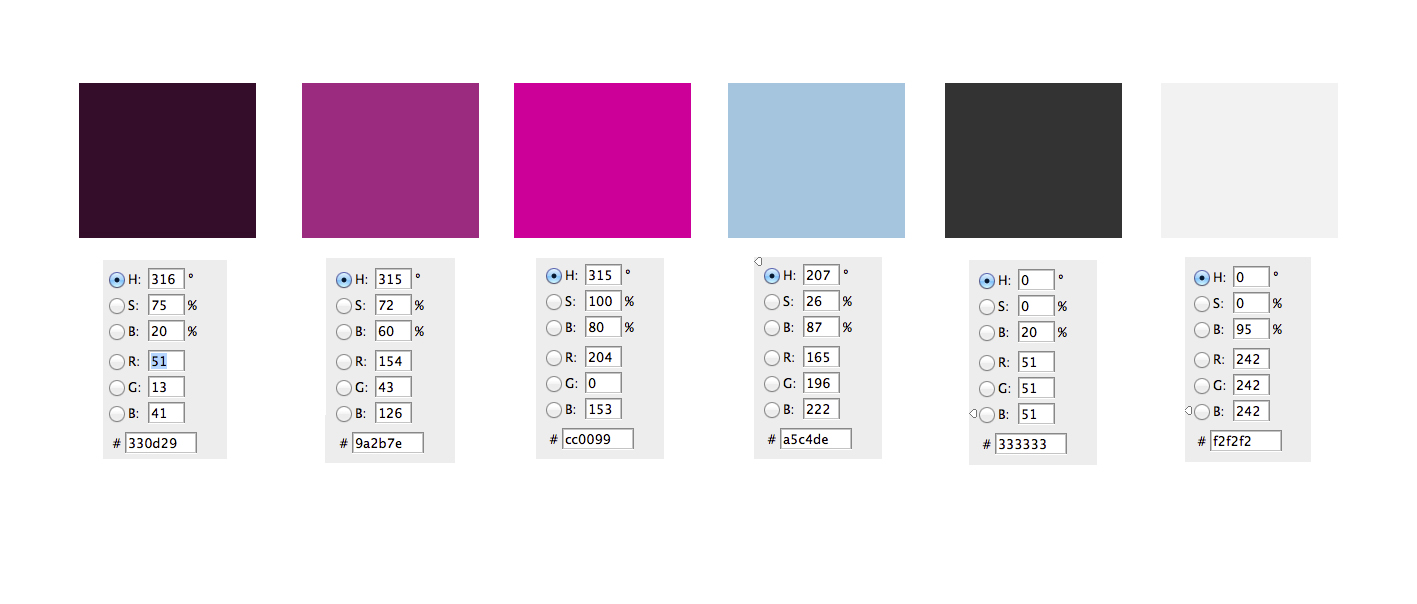
\includegraphics[scale=0.30]{../Figures/helsenorge_pallett.jpg}
\caption{Helsenorge color palette}
\label{figure:helsenorge-color-palette}
\end{figure}

\textbf{Retrieving the Data}

TODO

\textbf{Polling}

TODO

\section{Heart rate application}

TODO

\section{Weight application}

TODO

\section{Weight Polling Service}

TODO
